%%%%%%%%%%%%%%%%%%%%%%%%%%%%
\subsubsection{Physics Motivation}
\label{sec:sp-calib-sys-pns-phys} 

The supernova signal includes low energy (10~MeV) electrons, gammas; the final state will also include neutrons visible via capture. Such signals may be sensitive to (local) detector threshold effects, and energy scale, energy resolution; the requirements for these are 0.5~MeV, 1\%, 5\% respectively. Local detector conditions may change with time from a variety of 
%sources,
causes and include electronics noise, misalignments, fluid flow, and \efield. While these are intended to be characterized from other systems via inputs to the detector model, ``standard candles'' provide a method to assess if our detector model is incomplete or insufficient. An ideal ``standard candle'' matches one of the relevant signal processes. The Pulsed Neutron Source system, as described below, will provide a ``standard candle'' neutron capture signal (6.1~MeV multi-gamma) across the entire DUNE volume which is directly relevant to the supernova physics signal characterization.

%\fixme{SG: this intro needs fixing; our systems are not competing with each other, we need to present them as complimentary systems, so no need to say one is better than the other. I will edit this accordingly so the message is healthy for our maximum benefit.}


%In a TPC the energy reconstruction of a track depends on the amount of charge detected from electrons drifting from the track to the collection plane. For a fixed amount of ionization deposited at a point in the TPC, the amount of charge produced and collected depends on several factors: 
%\begin{enumerate}
%\item The local electric field strength affects the fraction of charge that recombines before drifting. The stronger the field, the less immediate recombination takes place, and thus the ratio of drifting electrons to energy deposited increases.
%\item The electron lifetime depends strongly on the purity of the argon liquid. Given the large size of the DUNE TPC, the restrictions to flow in the active volume, and a likely temperature gradient inside the liquid - it can be expected that there will be parts of the detecter where the electron lifetime will be shorter than others. The prediction of exactly how this manifests is difficult to predict {\it ab initio}.
%\item The distance electroncs have to drift to be collected depends on the location of the vertex inside the volume. The longer the drift, the more likeley it is an electron will be absorbed.
%\item Some parts of the detector can, in principle. be better or worse than others in terms of noise. This can affect the threshold charge collection systematically for different areas or the detector.
%\end{enumerate}

%Given these facts, it is highly desirable to be able to have a "standard candle" energy deposition of known energy that can be detected throughout the volume. Such a standard deposition would reveal variations in the local electron collection efficiency, especially if the source could be triggered such that the $t_0$ of the interaction was known.
%In principle, radioactive sources of known energy distribution could be deployed throughout the detector, but there are several problems with this approach: (1)  the source must be physically placed at the point one wishes to check, requiring multiple deployments in order to sample a significant volume of the detector, (2) the presence of the source itself can alter the electric field and ionization yield, and (3) the introduction of a foreign object into the active volume of the detector carries the risk of introducing impurities and/or radioactive contaminants. In addition, in order to have a triggered source (and hence some idea of $t_0$) one would have to introduce trigger electronics or other instrumentation - further complicating the deployment and increasing the risk.

%A way around this dilemma is to introduce short-lived radioactive atoms into the liquid argon itself, but this has the disadvantage  that there is no trigger and no way to ensure the standard candle decays spread out through the whole volume. In addition, to be useful such isotopes would have to have appreciable half-lives in order to have time to spread around the detector, and thus the whole process might take many hours. Finally, such isotopes would likely need to be made locally, which can be expensive and difficult.

%One way around these issues is to take advantage of a remarkable property of argon - the near transparency to neutrons with an energy near 57 keV due to an anti-resonance in the cross-section caused by the destructive interference between two high level states of the $^{40}$Ar nucleus. 
%As shown in Figure~\ref{fig:Arxsec}, 
%The cross-section at the anti-resonance "dip" is about 10 keV wide, and at the bottom the cross section of $1.6\times 10^{-4}\; b$ implies an elastic scattering length of over $2,000\;m$. Thus to neutrons of this energy the DUNE TPC is essentially transparent, and thus if injected from the top of the detector would reach energy part of the active volume. Of course, natural argon has three major isotopes: $^{36}$Ar (0.3336\%), $^{38}$Ar (0.0834\%), and $^{40}$Ar (99.6035\%) each with a slightly different anti-resonance. \\
%\begin{figure}[h]
%\begin{center}
%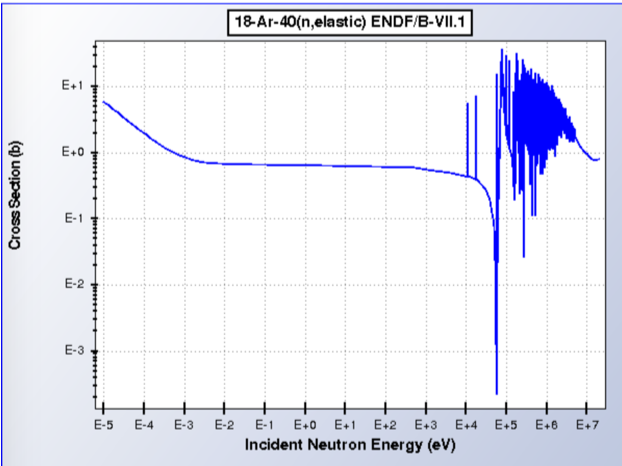
\includegraphics[width=0.4\linewidth]{Figures/Ar40xsec.png}
%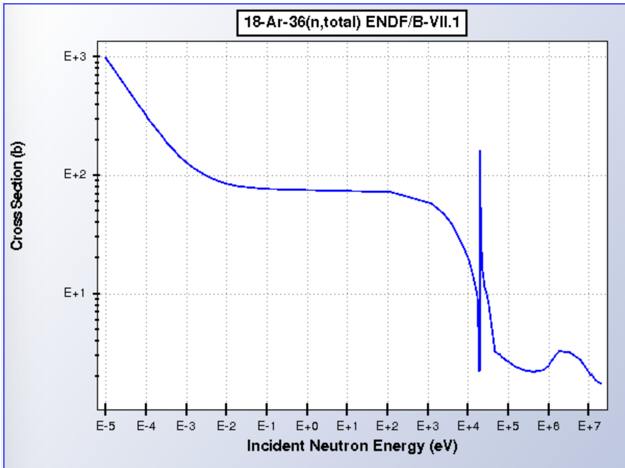
\includegraphics[width=0.4\linewidth]{Figures/Ar36xsec.png}
%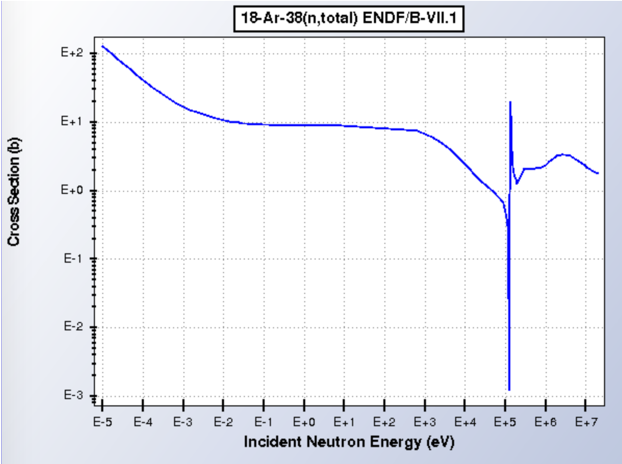
\includegraphics[width=0.4\linewidth]{Figures/Ar38xsec.png}
%\caption{Elastic scattering cross sections on 40-Ar (top left), 36-Ar (top right), and 38-Ar (bottom). From ENDF/B-VII.1~\cite{ref:ENDF}. The large anti-resonance at $57\; keV$ in 40-Ar can be clearly seen.
%{\bf NOTE: PUT IN PLOTS FOR ELASTIC}
%}
%\label{fig:Arxsec}
%\end{center}
%\end{figure}


%\begin{figure}[h]
%\begin{center}
%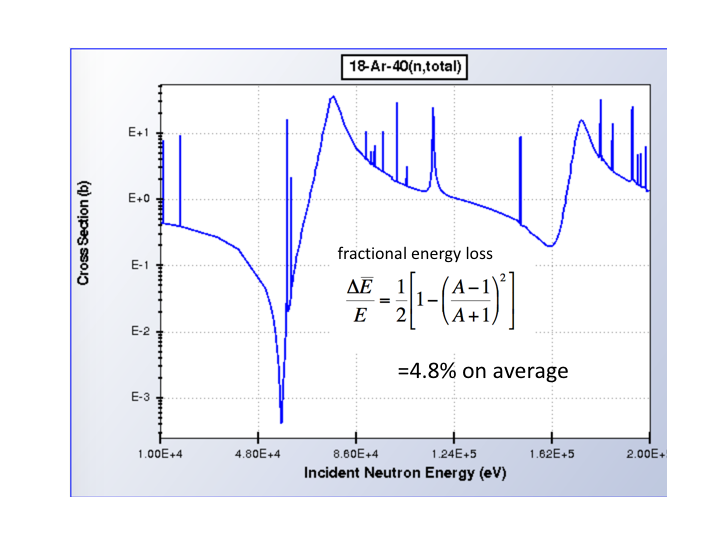
\includegraphics[width=0.75\linewidth]{Figures/Ar40Xsec2.png}
%\caption{Total scattering cross sections on 40-Ar in the range $10-200\; keV$~\cite{ref:ENDF}}
%\label{fig:Arxsec2}
%\end{center}
%\end{figure}

Liquid argon is near transparent to neutrons with an energy near or at 57~keV due to an anti-resonance in the cross-section caused by the destructive interference between two high level states of the $^{40}$Ar nucleus. The cross-section at the anti-resonance ``dip" is about 10~keV wide, and at the bottom the cross section of $1.6\times 10^{-4}\;$b implies an elastic scattering length of over $2,000\;$m. %Of course, natural 
Natural argon has three major isotopes: 36-Ar (0.3336\%), 38-Ar (0.0834\%), and 40-Ar (99.6035\%) each with a slightly different anti-resonance. The average elastic scattering length of the 57~keV neutrons in natural liquid argon is about $30\;$m.

The neutrons at the anti-resonance energy could be injected into liquid argon TPC, provided no material (e.g. hydrocarbons) blocks the path. Those that do scatter lose energy, leave the anti-resonance, quickly slow down and are captured. Each capture releases exactly the binding energy difference between $^{40}$Ar and $^{41}$Ar, about $6.1\; MeV$ in the form of $\gamma$ rays.  As will be described below, by using a {\it DD} Generator (where {\it DD} stands for "Deuterium-Deuterium"), a triggered pulse of neutrons can be generated outside the TPC, then injected via a dedicated hole in the insulation into the liquid argon, where it spreads through the 58~m volume of the detector to produce $6.1\; MeV$ energy depositions.
%Using this method, the calibration procedure would be quick (likely a few hours depending on the neutron yield of the DD generator), and there is no need to manufacture short-lived isotopes at an external facility.

The neutron capture $\gamma$ spectrum has been measured and characterized. Recently, the ACED Collaboration performed a neutron capture experiment using  the Detector  for Advanced  Neutron  Capture  Experiments  (DANCE)  at the  Los  Alamos  Neutron  Science  Center  (LANSCE). The result was published~\cite{aced} and will be used to prepare a database for the neutron capture studies.

%{\it Mention Test at LANSCE and its role?}

%%%%%%%%%%%%%%%%%%%%%%%%%%%%
\subsubsection{Design}
\label{sec:sp-calib-sys-pns-des}

The basic design concept of such a pulsed neutron source has been used successfully for Boron Neutron Capture Therapy\cite{KOIVUNORO2004853}. The design of the Pulsed Neutron Source used for energy calibration is shown in Figure~\ref{fig:PNS_Moderator}. The system will consist of four main components: a $DD$ generator, an energy moderator reducing the energy of the $DD$ neutrons down to the desired level, and the shielding materials, and a neutron monitor to confirm neutron flux and safe operation. 

\begin{figure}[tpb]
\centering
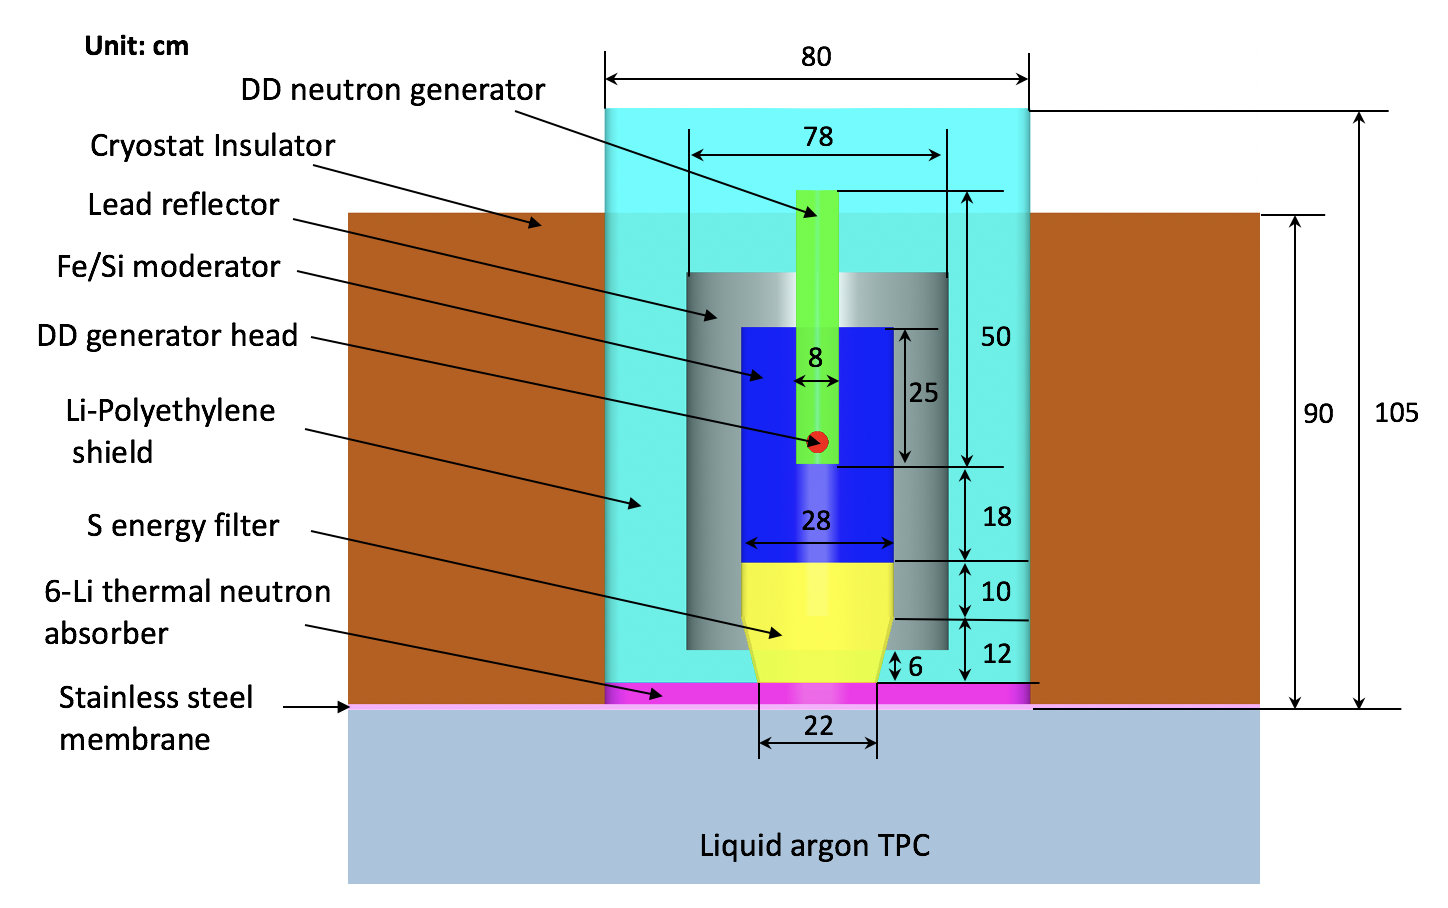
\includegraphics[width=12cm]{graphics/PNS_Moderator.png}
\caption{Conceptual design of the Pulsed Neutron Source. The whole device is placed outside the TPC volume on top of the cryostat.}
\label{fig:PNS_Moderator}
\end{figure}

{\bf DD generator source:} $DD$ generators are commercial devices that can be readily obtained from several vendors at a cost of about \$~125k each, which includes all control electronics. The pulse width is adjustable and can be delivered from about 10-1000~$\mu$s (which affects the total output). 

{\bf Moderator:}  A feasible moderator has been designed using a layered Moderator (Fe or Si)-Filter(S)-Absorber(Li) %layered 
configuration. The 2.5~MeV neutrons from the $DD$ generator are slowed down to below 1~MeV by the energy moderator. Natural iron and silicon are found to be efficient moderators for this purpose. Then an energy filter made of sulfur powder is used to further select the neutrons with desired anti-resonance energy.
The neutron anti-resonance energy in $^{32}$S is 73~keV, right above the 57~keV anti-resonance energy in $^{40}$Ar. The neutrons at this energy lose about 3.0~keV per elastic scattering length. After a few elastic scattering interactions, most of the 73~keV neutrons selected by the sulfur filter will fall into the 57~keV anti-resonance energy region in liquid argon. These materials require no cooling or special handling. Finally, a thermal absorbing volume of Lithium is placed at the entry to the argon pool in order to capture any neutrons that may have fallen below the 57~keV threshold. The reflecting volume is added around the $DD$ generator and the neutron moderator to increase downward neutron flux. 

{\bf Shielding:} The source will be encased in a shielding volume. The goal of the shield is to block both scattered neutrons and gammas which are produced in the source. Lithium-Polyethylene (7.5~$\%$) is chosen to be the material for the neutron shield because it is rich in hydrogen and lithium atoms which yield a high neutron absorption cross section. Lithium-Polyethylene is also light weight, commercially available, and relatively inexpensive. The energy spectrum entering the shield has multiple peaks between 0.5~MeV and 1.5~MeV, and one major spike at 2.2~MeV. The shield is able to effectively block the lower energy peaks but is only able to degrade the intensity of the 2.2~MeV peak. This is because 2.2~MeV gammas are a characteristic signature for neutron captures on hydrogen. A safe thickness of the lithium-polyethylene shield must be found such that it is capable of degrading the dose of 2.2~MeV gammas to safe levels. The dose of radiation from 2.2 MeV gammas was then calculated assuming a person standing 1~m away. Simulation indicates that 12~cm of Lithium-Polyethylene shield satisfies basic safety requirements. 

{\bf Neutron Monitor:} The system will need a monitoring system to confirm the source is operating as expected.  A neutron monitoring detector consisting of an Eljen EJ-420 coupled to an ADIT L51B16S 2-inch PMT will be placed just outside of the moderating material surrounding the $DD$ generator and will be read out with a CAEN waveform digitizer with neutron/$\gamma$ pulse-shape discriminating firmware. The monitoring detector will provide relative flux information to the calibration users and will ensure that the intensity of the source is constant, thereby allowing a comparison of data taking at different times.  A small collimator will be placed in front of the neutron detector, and inside the shielding material of the $DD$ source. The collimator dimensions and material specifications (likely a combination of iron, lead, and polyethylene) will be optimized from Monte Carlo simulations.

Based on the general concept, two different designs were studied with GEANT4 simulation. Figure~\ref{fig:PNS_source_design} shows a conceptual layout of the neutron injection system. %\todo{For v2, confirm updated figure; minor error in current one.}

\begin{figure}[tpb]
\centering
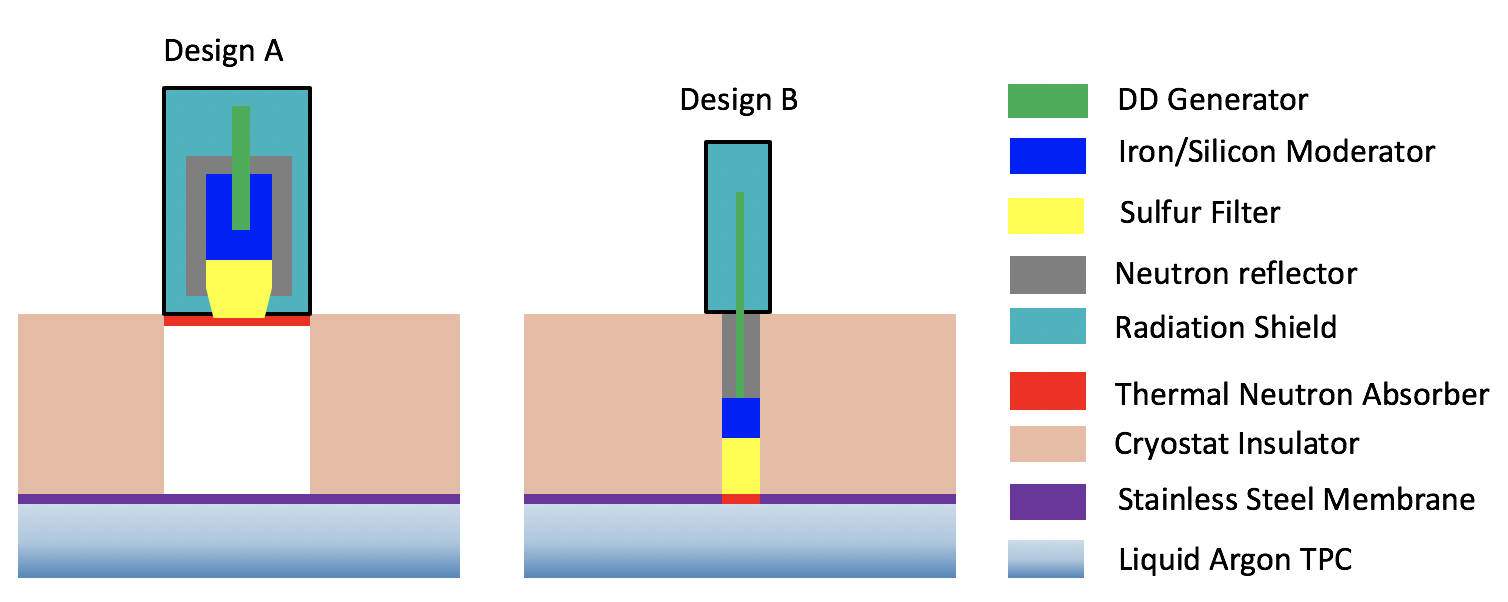
\includegraphics[width=16cm]{graphics/PNS_Two_Designs.png}
\caption{Two designs currently under development for the Pulsed Neutron Source. Design A: Large format neutron source to be deployed above/inside the human access holes or other delicate neutron injection ports; Design B: Small format neutron source to be deployed inside the calibration feedthrough ports.
%, see text for more details.
}
\label{fig:PNS_source_design}
\end{figure}

\begin{itemize}
\item Design A: Large format Moderator; \\
The neutron source is about 0.8~m wide and 1~m high. It would sit above the cryostat insulator. Beneath the neutron source, a cylinder insulator volume with a diameter of more than 50~cm has to be removed to allow the neutrons to get into the cryostat. Such an interface is provided by the human access ports near the endwalls of the detector; a picture of this is shown for \dword{protodune} in Figure~\ref{fig:humanaccessport}. The top flange is sealed, and the neutron source sits on top (Design A), providing heat insulation; The neutron source weighs about 1.6~tons and will hang on the I-beam supporting structure. This design allows a permanent deployment of the neutron source. GEANT4 simulation has shown that 0.13 ~\% of the neutrons generated by the $DD$ generator are expected to be captured inside the liquid argon TPC. It is also possible to place the neutron source inside the human access port which would allow a factor of 6 increase of the neutron flux but require a modification of the interface flange. This is currently being investigated.
% JW: I think It doesn't harm to mention that the neutron source could be placed inside the manhole. My recent simulation is based on this configuration.

%\item \fixme{KM: I do not think this is possible for quite a few reasons-- heat loss and also cost of adjusting this. Remnoving this for now.} Design B: Large format Moderator; no insulation between Moderator and cryostat membrane The design of the the neutron source itself would be same as Design A. The only difference is that the neutron source will be placed inside a hole on the cryostat insulator. The cryostat will be kept closed, but there is no vacuum insulation between the neutron moderator and the stainless steel membrane. As the neutron source is closer to the liquid argon cryostat, the neutron flux is expected to be a factor of 10 higher than that of Design A. However, the neutron source must be removed and the insulator has to be recovered after the calibration run. 
\item Design B: Small format Moderator; no insulation between Moderator liquid argon. An alternative method for delivering the neutrons is to use the existing calibration feedthroughs. In the current cryostat design, 20 calibration feedthroughs with a 20~cm inner diameter will be available on top of the cryostat. One can design the neutron source with an ultra-thin $DD$ generator that fits the size of the feedthrough. The problem is that there will be no space in the feedthrough for the shielding materials to fit in, so additional shielding will need to be placed around the feedthrough. The weight of this compact neutron source will be about 140~kg, so mounting will be simpler compared to Design A. The effective neutron flux is expected to be similar as that of Design A. 
\end{itemize}

\begin{figure}[tpb]
\centering
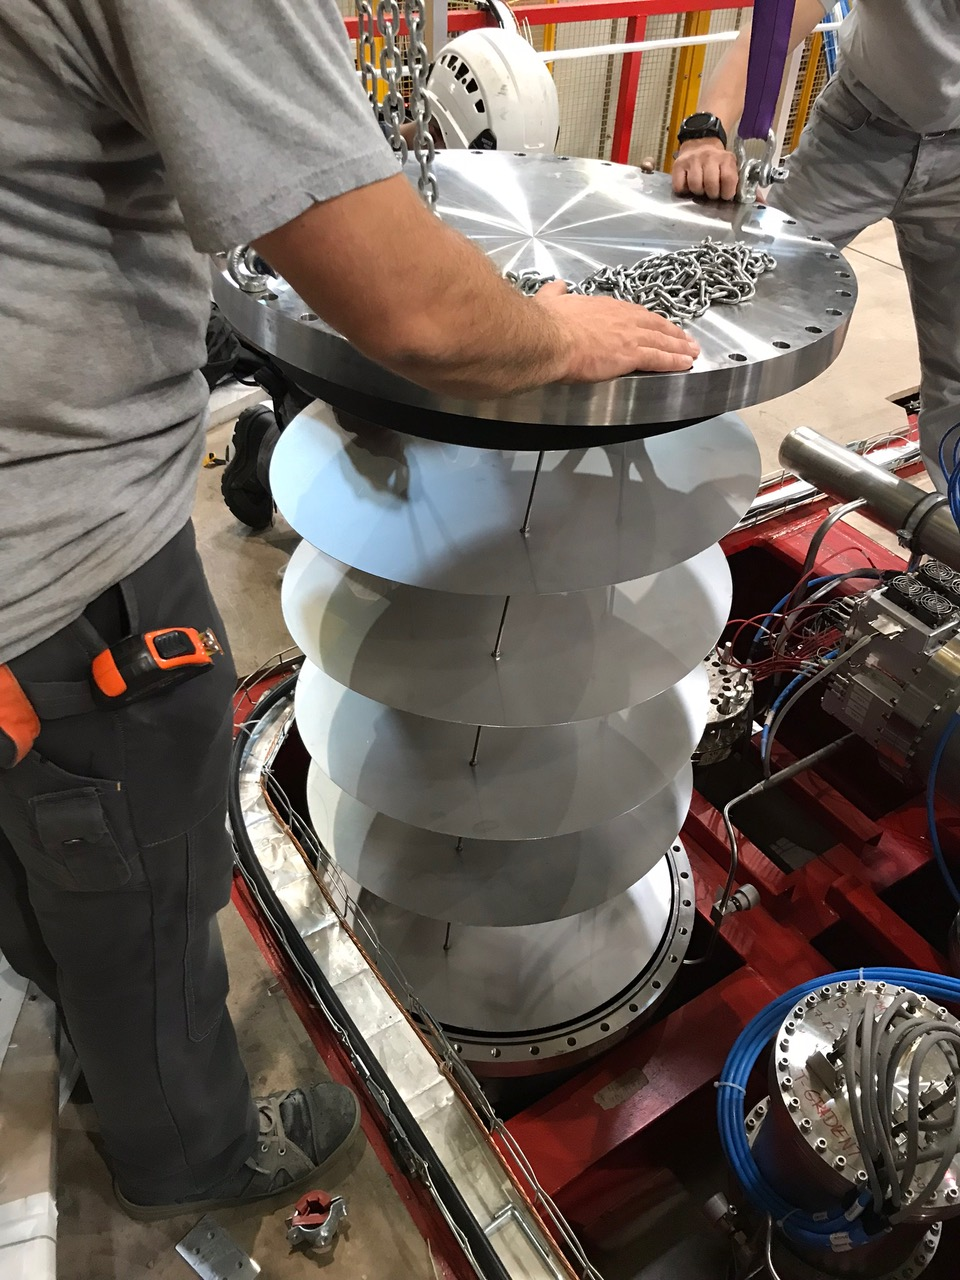
\includegraphics[width=6cm]{graphics/manhole2.jpg}
\caption{Flange for human access port on ProtoDUNE-SP and support structure (red frame).}
\label{fig:humanaccessport}
\end{figure} 

\begin{figure}[tpb]
\centering
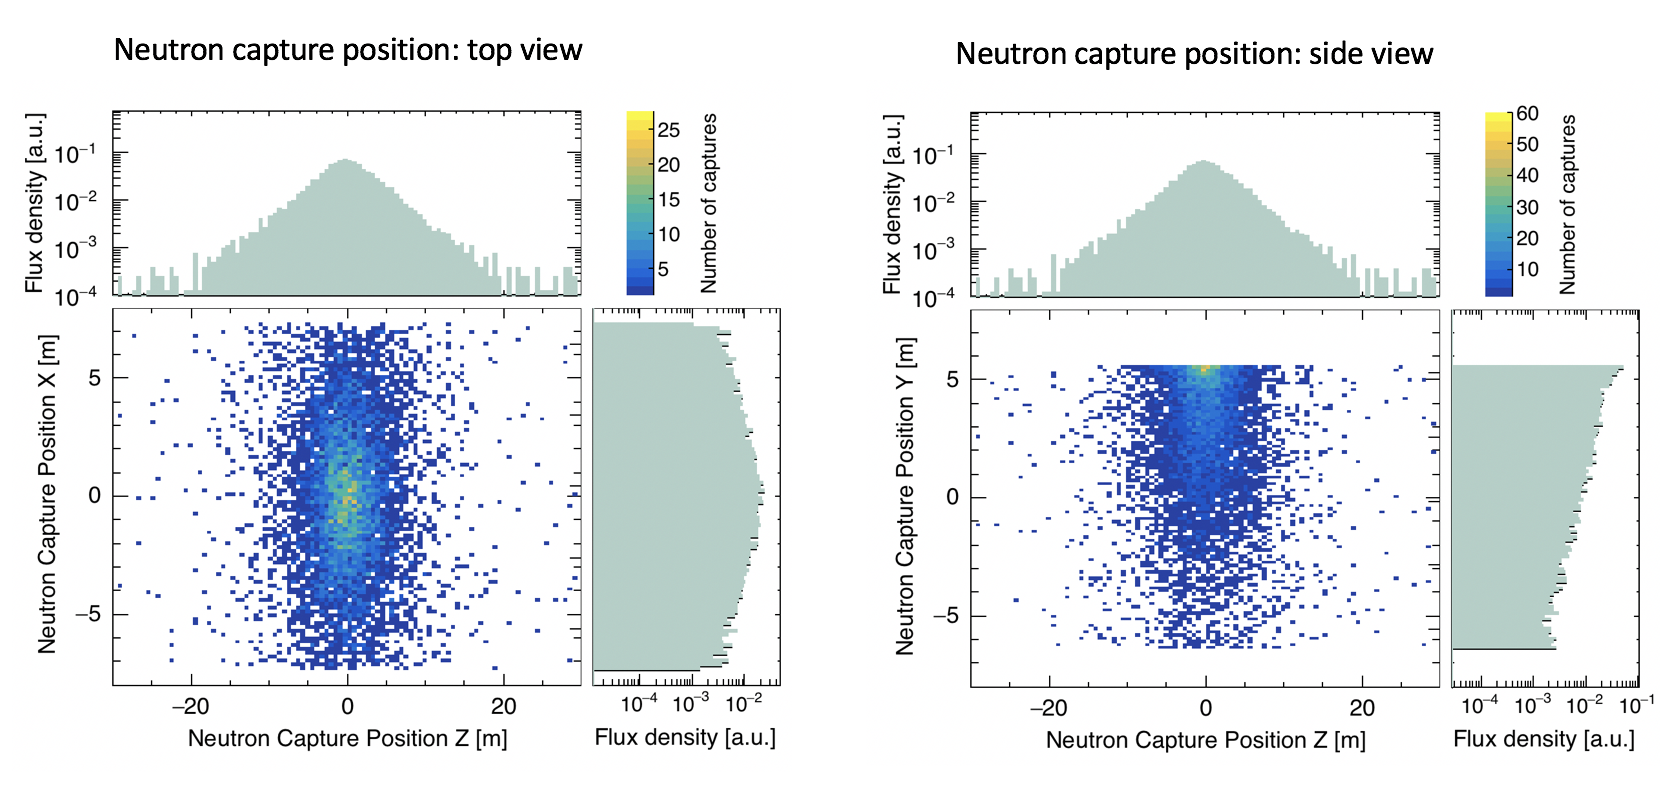
\includegraphics[width=18cm]{graphics/PNS_NcapPosition.png}
%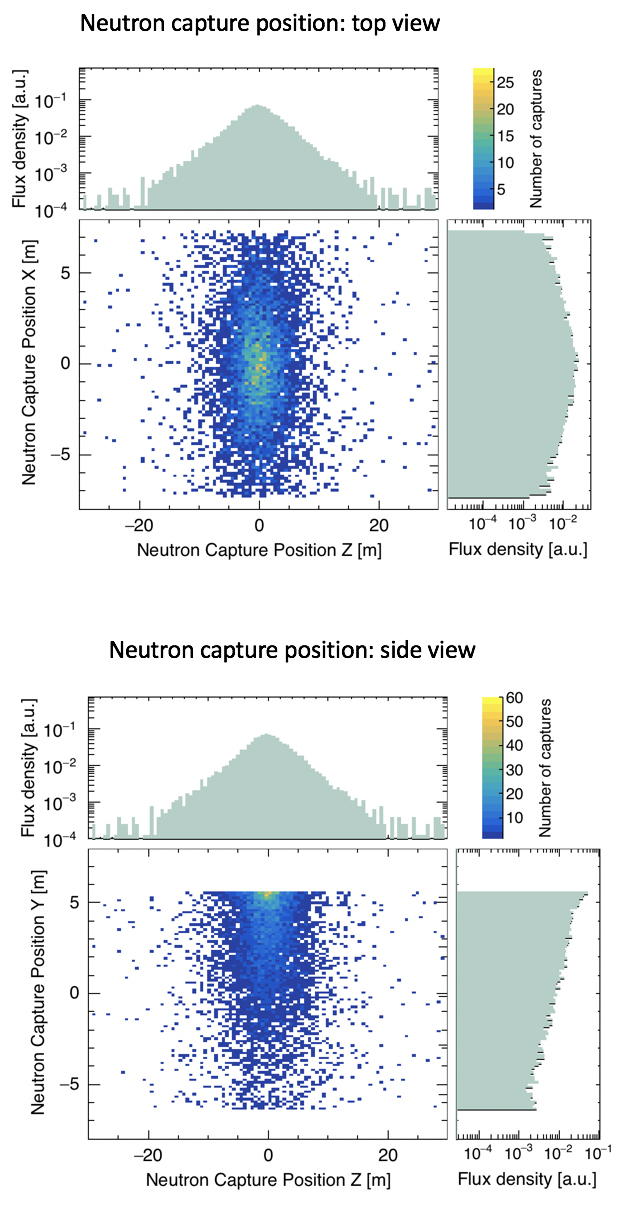
\includegraphics[width=10cm]{graphics/PNS_NcapPosition_v2.png}
\caption{Neutron capture positions inside a DUNE sized TPC. L=60~m (along Z axis, horizontally parallel to the beam direction), W=14.5~m (along X axis, horizontally perpendicular to the beam direction), H=10~m (along Y axis, vertically perpendicular to the beam direction). The neutron moderator is based on Design A, but the entire source is placed inside the injection port that is central to the cryostat. 10$^{6}$ DD generator neutrons with 2.5~MeV energy were simulated in the moderator and propagated inside the liquid argon TPC. Left: Top view of neutron capture positions. Right: Side view of neutron capture positions.} 
\label{fig:ncapposition}
\end{figure} 

The two designs were simulated in GEANT4. The position distribution of the neutron captures is shown in Fig.~\ref{fig:ncapposition}. In the simulation, the Pulsed Neutron Source is placed on top of the liquid argon cryostat with the same size as the DUNE 10~kton TPC. Initial simulation results indicate that one Pulsed Neutron Source could cover half the TPC volume, so two identical neutron sources, each central to half the cryostat top,  %\todo{SG: I assume this is with design A, right? if so, mention which design}
would illuminate the whole TPC volume of the DUNE far detector for both designs. However, this would require opening two additional neutron injection ports which are not included in the current cryostat design \footnote{Ideally,opening two identical neutron injection ports for each 10~kton TPC would make full use of the neutron source. The possibility requires further discussion with the cryostat engineers.}. Alternatively, two large format neutron sources (Design A) could be permanently deployed at the human access holes at the corners of the cryostat. One concern is that the neutrons scattered from the liquid argon volume from the human access holes may not reach the center of the TPC. This can be mitigated by using a small format neutron source (Design B) deployed on top at the center of the cryostat using the multi-purpose feedthroughs. %could be used to complement the coverage of the large format sources. 
Figure~\ref{fig:PNS_energy_design} shows the energy spectrum of the neutrons moderated and injected to the liquid argon TPC, based on Design A.
% This figure is based on Design A moderator placed inside the manhole. We can still use this figure, because the energy spectrum shape should be same. Only the flux will be a factor of 6 lower
%The neutron energy is moderated from 2.5 MeV to below 100 keV.  

\begin{figure}[tpb]
\centering
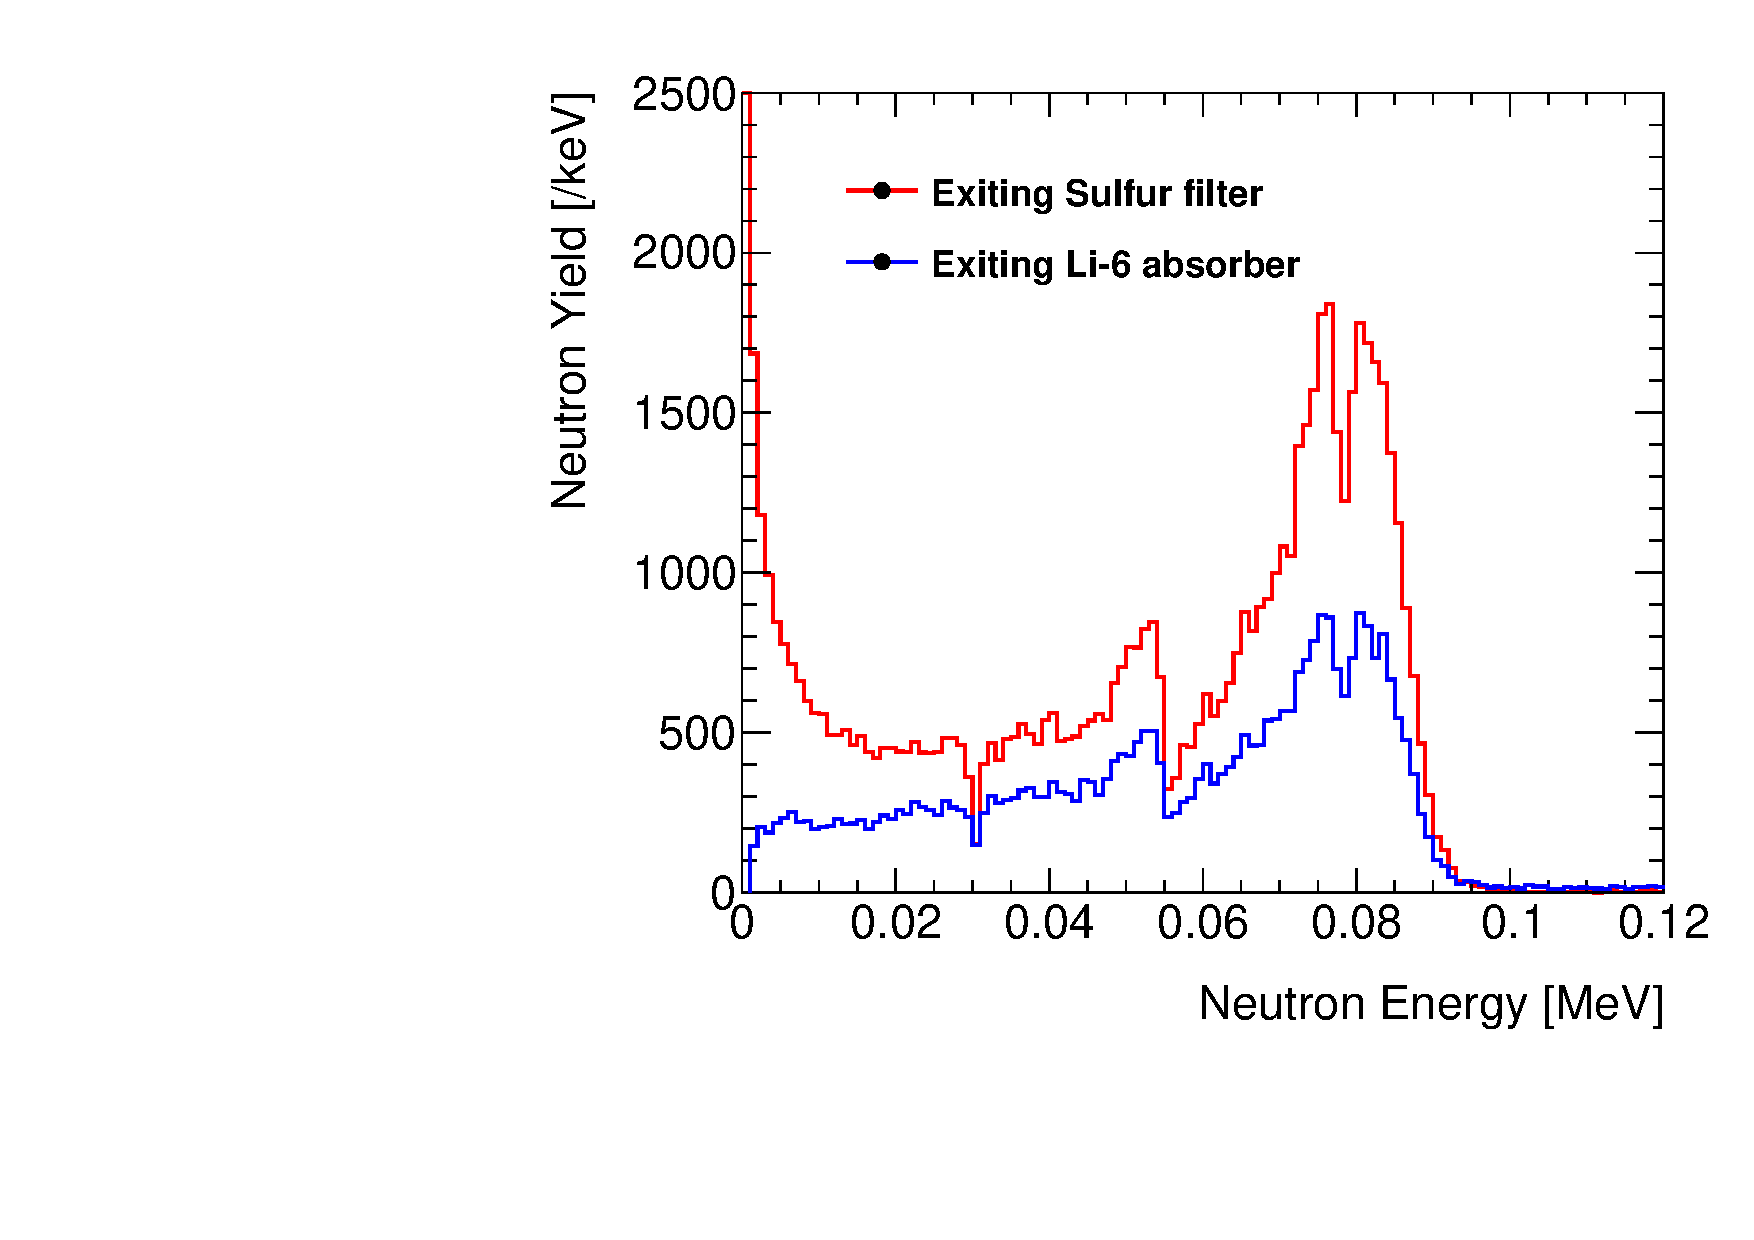
\includegraphics[width=10cm]{graphics/PNS_Energy_Moderator.pdf}
\caption{Energy of moderated neutrons produced by the Pulsed Neutron Source. Simulation is based on Design A. The total number of initial DD generator neutrons is 10$^{6}$ }
\label{fig:PNS_energy_design}
\end{figure} 

The system is expected to have a long lifetime of operation, but as the PNS system sits on top of the cryostat, with no opening to the liquid argon, it is possible to replace the system if it fails with only crane support.


%%%%%%%%%%%%%%%%%%%%%%%%%%%%
\subsubsection{Possible Measurements}
\label{sec:sp-calib-sys-pns-meas}

The 6.1~MeV $\gamma$ cascade will provide a uniform signal for neutron capture, part of the supernova signal. The source may also be used determine the relative efficiency across the detector for neutron capture, and also provide measurements of energy resolution and energy scale spatially and temporally resolved. Simulation studies are currently underway and for the second draft, we plan to include a first round of simulation results.

%\todo{Simulation studies are underway but changing rapidly. for v2 we will include a first round of studies.}





